\documentclass[11pt]{report}
\usepackage{outline}
\usepackage{pmgraph}
\usepackage{graphicx}
\usepackage[normalem]{ulem}
\title{\textbf{Project Report}}
\author{Enigma\\ Tanuj Kaza \\ Harsh Bansal \\ Bhavya Bahl \\}
\date{\oldstylenums{05}/\oldstylenums{11}/\oldstylenums{16}}
\setlength{\oddsidemargin}{0in}
\setlength{\evensidemargin}{0in}
\setlength{\topmargin}{0in}
\setlength{\headsep}{-.25in}
\setlength{\textwidth}{6.5in}
\setlength{\textheight}{8.5in}
\setlength{\parindent}{1cm}
\graphicspath{ {images/} }

\begin{document}
\maketitle 

\begin{abstract}
Feeder was started by a group of IIT Bombay sophomores with a view to changing how courses function in their institute(and elsewhere). It is meant to bridge the communication gap between the students and the professors which in turn will improve the quality of the course being dished out. \\

The instructors can receive constructive feedback on various aspects of the course and can thus dynamically change the ocurse structure for the better. The students too are sent reminders for the assignments and deadlines so that they do not miss out on important submissions and can plan their schedule more effectively.
\end{abstract}

\newpage
\begin{outline}
	\item Design
	\begin{outline}
		\item The project is built on a Django Framework
		\item The student interface is an Android Application
		\item The android application uses the django server as the backend server
		\item The App uses Bootstrap for styling and for embellishing the user interface of the application
		\item The ReportLab and Imaging Libraries of python are used for generating graphs
	\end{outline}
\end{outline}
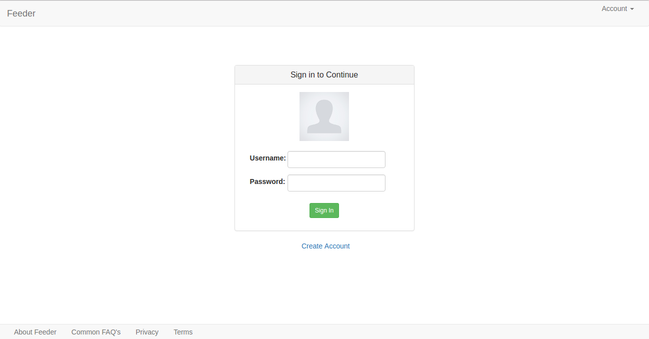
\includegraphics{Home}

\newpage
\begin{outline}
	\item Features and Technical Details
    \begin{outline}
    	\item Admin Features
    	\begin{outline}
    	\item Admin can add students into courses from a list of enrolled students
\item The list of students is imported from a csv file named 'student.csv' when the admin logs in. If there are any new students in the csv file, then even they will be added to the database
\item The other functionality for the admin is adding courses. The fields in the add course form are mandatory and must be filled. The year field must be an integer(example : 2016). Apart from that Department is selected from the list of departments in IIT Bombay.
\item Now the instructors must be selected for this course. There is a many to many mapping from instructors to course. One course can have multiple instructors(eg.MA105 and other freshmen courses, or consider an instructor and the Teaching Assistants(TA's) for the course. The TA's are treated as instructors in this app.). So all the instructors taking this course must be selected form the multiple select list.
\item Following this, the admin is prompted for midsem and endsem deadlines(It is not compulsory that the admin adds a midsem or endsem deadline and hence functionality has been provided where he can move directly to the feedback forms)
\item Some courses like CS101 in first year have multiple endsem and midsem examinations(Lab and theory courses). Hence functionality has been provided for the admin to add multiple midsem and endsem deadlines.
\item The midsem and endsem deadline buttons are toggle buttons and can be clicked if you realise you do not want to add a deadline
\item In the feedback form, there are some default objective questions(Questions which will have answers in the form of ratings from 1:5) and some subjective questions(Subjective Text Questions). 
\item In addition to that, the admin can remove some of these questions, and add some more default questions which have been provided. In addition to this, the admin can also add some of his own objective and subjective questions(Not required, but he has been provided the functionality!). After all questions have been added, he has to add a feedback deadline and then he progresses to the endsemester form.(Where similar functionality is provided)Thus we have customized Feedback Forms
\item Apart from this we have a privacy policy and a terms of service too[Links given in the footer](Source has been cited) to which we strictly adhere to :P
\end{outline}

\newpage
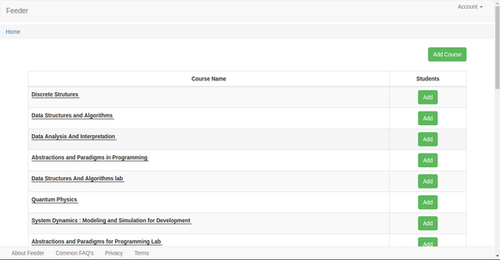
\includegraphics{admin_home} \\ \\ \\ \\ \\
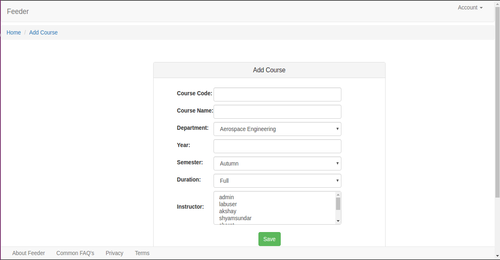
\includegraphics{add_course}

\newpage
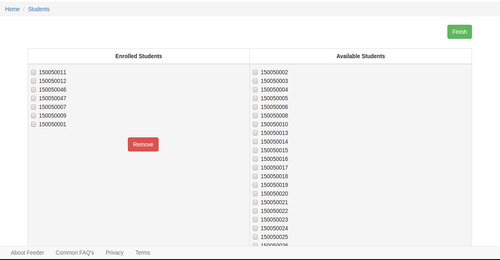
\includegraphics{add_student}   \\ \\ \\ \\ \\
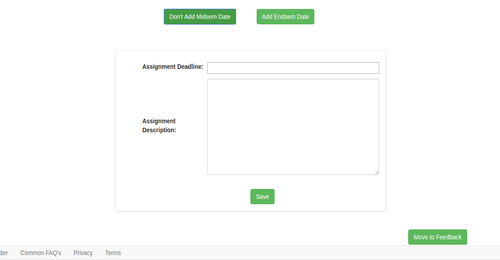
\includegraphics{add_deadline} 

\newpage
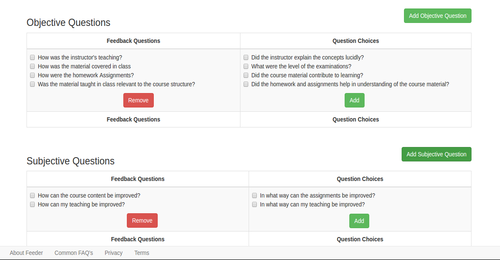
\includegraphics{add_feedback}   \\ \\ \\ \\ \\
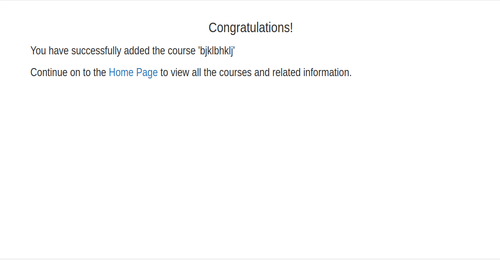
\includegraphics{congrats} 

\newpage
    	\item Instructor Features
    	\begin{outline}
    	\item Once you login with any of the above mentioned credentials, there are a list of courses being taken by the instructor and the ability to add assignments and feedback forms in each of the courses. The courses can be viewed by only the instructor taking the course and the Teaching Assistants for that course
    	\item The assignments can be seen in the form of deadlines pending and those that have been completed, with the capability of editing the assignment fields(Deadlines,specifications.etc). The Feedback can also be seen on the same page. This makes for a compact application.
    	\item Assignments can be added into each course[Foreign Key Relationship] in real time with the provision for adding deadlines and specifications
		\item The instructor can also view the feedback that has been submitted by the students, in interactive formats like graphs for objective questions(As well as in aggregate format) and the subjective results are also in aggregate format.We have used The ReportLab and the Imaging Libraries for showing the graphs
		\item In the feedback form, there are some default objective questions(Questions which will have answers in the form of ratings from 1:5) and some subjective questions(Subjective Text Questions). This accounts for all types of questions
		\item There is a many to many field relationship between feedback questions and feedback forms. There is a foreign key from feedback answers to feedback questions and feedback forms. Hence each answer is uniquely identified
		\item In addition to that, the instructor can remove some of these questions, and add some more default questions which have been provided. In addition to this, the instructor can also add some of his own objective and subjective questions(Not required, but he has been provided the functionality!). After all questions have been added, he will be redirected to the course page.
		\item The instructor can add as many feedback forms as desired.
		\item We have provided facebook login for the instructors
		\item You can click on the feeder brand name in the top left corner to be directed to the home page.
\end{outline}

\newpage
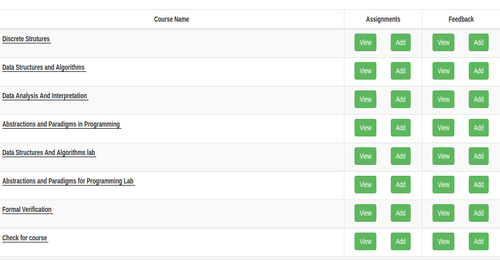
\includegraphics{instruct_home}   \\ \\ \\ \\ \\
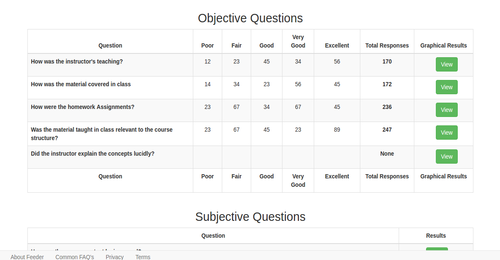
\includegraphics{o_feedback} 

\newpage
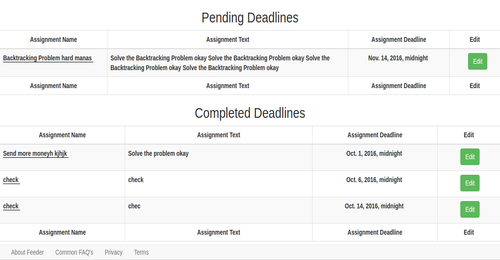
\includegraphics{deadlines}   \\ \\ \\ \\ \\
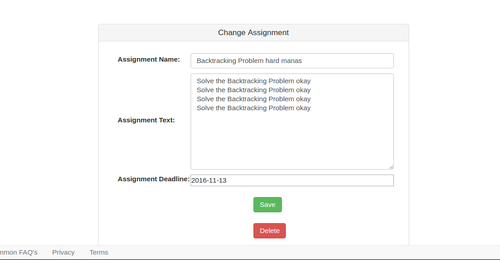
\includegraphics{deadline} 

\newpage
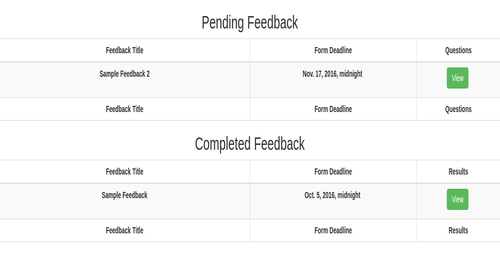
\includegraphics{feedback}   \\ \\ \\ \\ \\
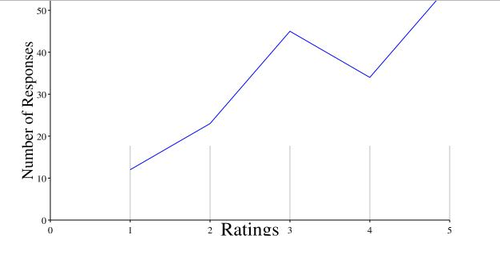
\includegraphics{graph} 

\newpage
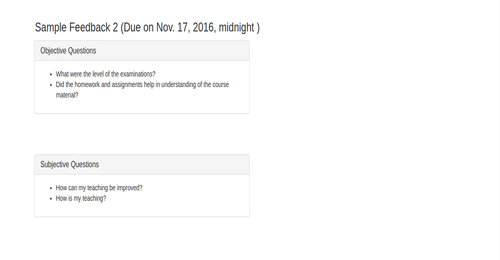
\includegraphics{s_feedback}   \\ \\ \\ \\ \\


	\item Student Interface
    \begin{outline}
    	\item The authentication to the django server was a main hurdle for us in this task
    	\item Once the student logs into the app, he sees a calendar view which has the different days which are colur coded on the basis of assignments and deadlines
    	\item He is also able to see a feedback form
    	\item A logout feature has been provided
    	
	\end{outline}
\end{outline}
\end{outline}

\newpage
\textbf{Reflection Essay} \\ \\
This project was the first major project for most of us and certainly on which taught us a lot. Having built websites only in plain-old PHP prior to this, a web framework like Django was a lot easier once we understood how it worked and we got the hang of it. Django has a lot of functionality and very little code is required for it, and this is just what we need in this day and age.

	We learnt how to develop user friendly portals, interactive UI and many mnay other features that Django provides.

	Regarding Social Login, we hit a brick wall when we tried to do login for Gmail using their API. We spent a lot of time on this before we eventually gave up on Gmail Login and attempted to do facebook login at which we succeeded. In hindsight, this time could have been used more wisely.

	Coming to Android, even here we spent almost a whole week trying to do the authentication using oauth and not just plain java. Oauth being more secure was the preferred choice, and although we tried and tried, we finally had to resort to Java to do what we had to do. This I believe was the main reason for not being ablke to complete all the features of the Android Student Interface.
	Some learnings from the Android Project:-
	\begin{itemize}
	\item	Can’t use same intent definition in two different functions.
	\item Get-Post along with Django views makes client-server interaction between them.
		== is not commonly used in Java. object1.equals(object2) is preferred.
		Internet requests better be in Background Threads(“implemented using Async task”), prefer not to use any variable whose value is 	expected from the thread in our Main thread.
	\item Shared Preferences:- Usage(helped by Lohith)This project was the first major project for most of us and certainly on which taught us a lot. Having built websites only in plain-old PHP prior to this, a web framework like Django was a lot easier once we understood how it worked and we got the hang of it. Django has a lot of functionality and very little code is required for it, and this is just what we need in this day and age.

	We learnt how to develop user friendly portals, interactive UI and many mnay other features that Django provides.

	Regarding Social Login, we hit a brick wall when we tried to do login for Gmail using their API. We spent a lot of time on this before we eventually gave up on Gmail Login and attempted to do facebook login at which we succeeded. In hindsight, this time could have been used more wisely.

	Coming to Android, even here we spent almost a whole week trying to do the authentication using oauth and not just plain java. Oauth being more secure was the preferred choice, and although we tried and tried, we finally had to resort to Java to do what we had to do. This I believe was the main reason for not being ablke to complete all the features of the Android Student Interface.
	Some learnings from the Android Project:-
	(
		Can’t use same intent definition in two different functions.
		Get-Post along with Django views makes client-server interaction between them.
		== is not commonly used in Java. object1.equals(object2) is preferred.
		Internet requests better be in Background Threads(“implemented using Async task”), prefer not to use any variable whose value is 	expected from the thread in our Main thread.
		Shared Preferences:- Usage(helped by Lohith) ->
		1. SharedPreferences sharedprefs = this.getApplicationContext();
		2. sharedprefs = getSharedPreferences(“Name for reference”,0(or 1,2,..)) // (int string,int mode)
	)

	All in all, a good project. \\ 
		1. SharedPreferences sharedprefs = this.getApplicationContext(); \\ 
		2. sharedprefs = getSharedPreferences(“Name for reference”,0(or 1,2,..)) // (int string,int mode)
	) \\ 
	\end{itemize}
	All in all, a good project.
\end{document}